\documentclass{article}
\usepackage{realtristan}
\title{Chemistry}
\author{Tristan Simpson}
\begin{document}
\maketitle
\tableofcontents

\section{Atoms and Molecules}
\begin{itemize}
    \item An atom is the smallest unit of an element.
    \item A molecule is a group of same elements bonded together.
    \item A compound is a group of different elements bonded together.
\end{itemize}

\section{Inter and Intramolecular Forces}
\begin{itemize}
    \item The \textbf{intramolecular} force is what holds the elements together.
    \item The \textbf{intermolecular} force is what holds the compounds (a group of atoms bonded together) together.
\end{itemize}
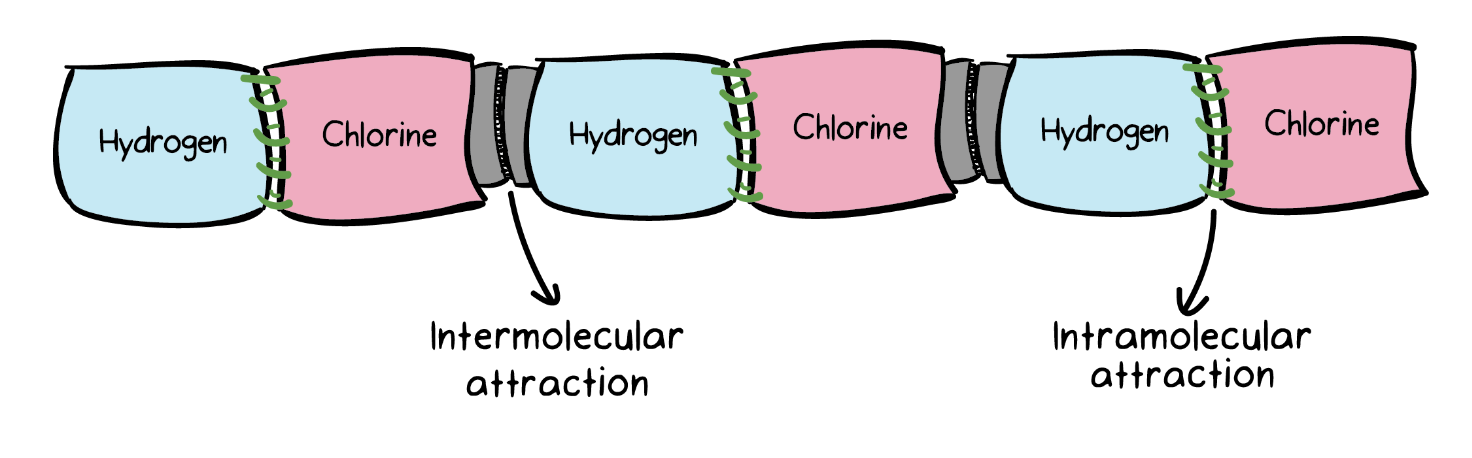
\includegraphics[scale=0.33]{images/molecularforces.png}

\subsubsection{Atomic Chemistry Review}
\begin{itemize}
    \item The nucleus of an atom is made up of protons (+ charge) and neutrons (- charge). An isotope of an element is when an atom's nucleus has a different number of neutrons to protons (The number of protons is the elements atomic number). Neutrons can be removed by supplying the atom with enough energy for the \hyperref[sec:nucleon]{nucleon} to be removed
    \item The electrons (- charge) orbit the nucleus in a circular motion. The number of electrons for a neutral atom is equal to the number of protons. By adding an electron, the atom becomes negatively charged, by removing an electron, the atom becomes positively charged. The electrons are distributed by the Bohr Rutherford Diagram (Shown \hyperref[sec:electronwaves]{here}).
    \item Depending on the number of electrons removed/added, the charge varies. (i.e. remove 2 electrons, the charge is +2, remove 1 electron, the charge is +1, add 1 electron, the charge is -1, add 2 electrons, the charge is -2, and so on...)
    \item A positively charged ion is called a Cation. A cation is formed when an electron is removed.
    \item A negatively charged ion is called an Anion. An anion is formed when an electron is added. (Remember, an electron is negative, therefore adding another negative charge just makes something more negative)
\end{itemize}\leavevmode\\

\subsubsection{Bohr Rutherford Diagram}
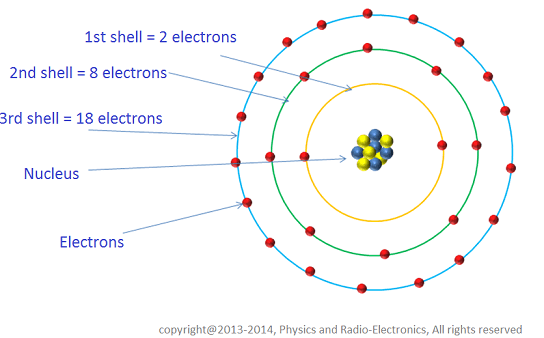
\includegraphics[scale=0.5]{images/atom_orbitals.png}\label{sec:atomorbitals}

\end{document}